\section{Concepts}
\label{sec:concepts}
This section describes the conceptual design of the multi-agent troubleshooting system. While
\cref{sec:background} introduced the underlying technologies in general terms, this section explains
\emph{how} these concepts are applied to the problem of network troubleshooting and, more importantly,
\emph{why} the system is designed the way it is. The realisation (implementation) in code is deferred to
\cref{sec:implementation}, and the experimental procedure used to evaluate the design is described in
\cref{sec:methodology}.


\subsection{Scope: Two Independent Parts}
\label{sec:concepts-scope}
The work described in this report consists of two distinct and largely independent parts, which it is
important to keep apart conceptually.

The \emph{first part} is the core of the project and addresses the research questions stated in
\cref{sec:introduction}: which network problems can be troubleshooted by a multi-agent system, with what
success rate across difficulty levels, and at what cost. This part is driven by a human operator who poses a
troubleshooting goal to the user-facing orchestrator, and it is evaluated quantitatively against a catalogue
of reproducible fault scenarios (see \cref{sec:evaluation-concept,sec:model-tier-concept}). The bulk of the
architecture, the agent roles and the evaluation concept described below serve this first part.

The \emph{second part} is an independent feasibility use case rather than a measured research question: the
\emph{automatic syslog investigation}. The motivating question here is not \emph{how well} or \emph{at what
cost}, but simply \emph{whether} it is possible to build a system that reacts autonomously to certain syslog
messages and starts a self-contained initial investigation without any human trigger. How such a mechanism works in
practice and how a human operator can take over and continue the troubleshooting without
repeating the work the autonomous investigation has already done. This use case reuses the same
agents shown and described in \cref{fig:architecture-overview} building blocks but it uses a different entry point (\texttt{investigation\_orchestrator}). It is described on its own in
\cref{sec:autonomous-syslog-usecase} and is not part of the quantitative evaluation.

\subsection{Overall Architecture}
\label{sec:architecture}
The system is structured as a \emph{hierarchical}, \emph{role-based} multi-agent system, the collaboration
pattern introduced in \cref{sec:multi-agent}. A central \emph{orchestrator} agent receives a troubleshooting
goal and delegates focused sub-tasks to a set of specialised sub-agents, each responsible for one domain of
the network (see \cref{sec:agent-roles}).

The decisive reason for distributing the work across several agents rather than handling it in a single,
monolithic agent follows directly from the limitations discussed in \cref{sec:tokens-context-cost}. A single
agent would have to hold the entire troubleshooting context (all tool definitions, all device output, the full
conversation history) in one large context window. This both approaches the hard context limit and
degrades output quality through the "lost in the middle" effect. By contrast, each specialised agent receives
only a focused instruction set and a small, domain-scoped selection of tools, which keeps its individual
context small and reduces context-related quality degradation.

Each agent in this architecture is an independent agent loop (see \cref{sec:agent-loop}), it runs its own
loop over its own context and tool set, driven by the same underlying agent harness. Delegation is itself realised as a
tool call, the orchestrator's loop invokes a sub-agent as a tool, the sub-agent runs its own loop to completion and
returns its findings, which the orchestrator then incorporates into its own context.

\Cref{fig:architecture-overview} shows the resulting architecture: the orchestrator at the top delegates
domain-scoped sub-tasks to the specialised sub-agents, each of which has its own tools.

\begin{figure}[htbp]
\begin{center}
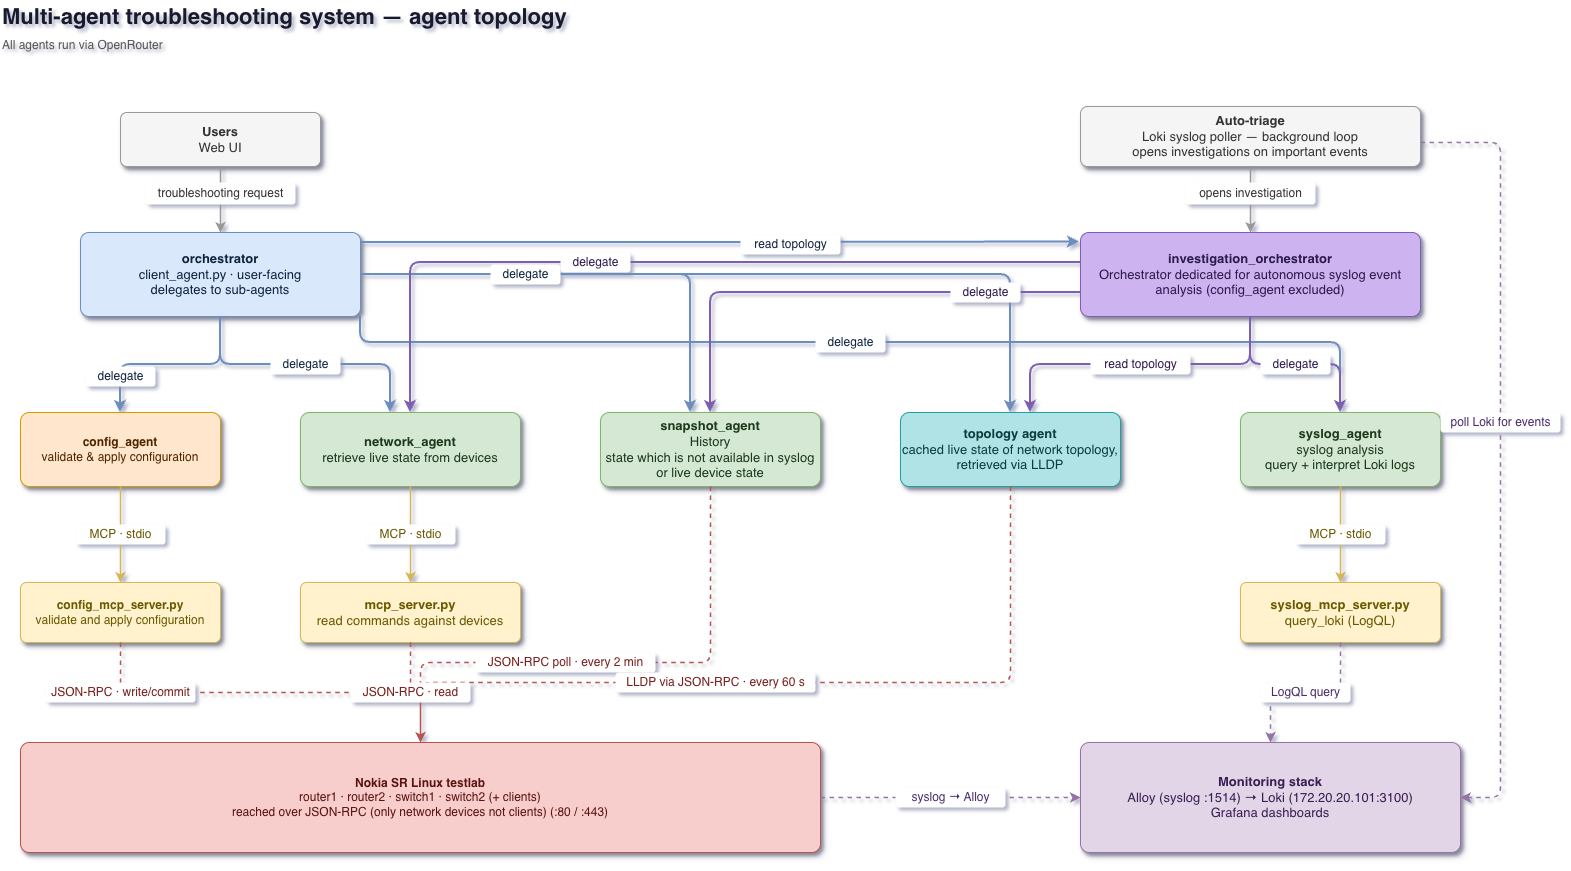
\includegraphics[width=0.9\linewidth]{graphics/agents-architecture.png}
\end{center}
\caption{Architecture of the multi-agent troubleshooting system.}
\label{fig:architecture-overview}
\end{figure}

\subsection{Agent Roles and Responsibilities}
\label{sec:agent-roles}
Each agent has a single, defined responsibility and a deliberately limited scope. The following roles make
up the system:

\begin{itemize}
    \item \textbf{Orchestrator (user-facing).} Coordinates an interactive troubleshooting session, splits
          the user's goal and delegates sub-tasks to sub-agents and synthesises their findings into a final answer. Since the sub-agents are "stateless" the orchestrator
          needs to supply all the required information to the sub-agents.
    \item \textbf{Investigation orchestrator (autonomous).} Coordiantes the autonomous syslog event based investigations. 
          It runs the same delegation pattern as the user-facing
          orchestrator without access to the config agent.
    \item \textbf{Network agent.} Retrieves live device state through read commands.
    \item \textbf{State-snapshot agent.} Provides historical device state. The state-snapshot agent focuses on information which can't be retrieved via syslog or
          device life state but can be useful for troubleshooting (like past ARP entries or routing tables).
    \item \textbf{Topology agent.} Supplies the (cached) network topology so other agents can reason about how
          devices are connected. It compares the "should be" state of the topology with the actual "live" state of the network (via LLDP queries).
    \item \textbf{Syslog agent.} Queries and analyses syslog data for the entire network.
    \item \textbf{Configuration agent.} The only agent with \emph{write} access. It is able to apply
          configuration changes to devices.
\end{itemize}

\subsection{Tool and Capability Layer}
\label{sec:tool-layer}
Agents gain the ability to interact with the outside environment through the function-calling mechanism described in
\cref{sec:func-calling}, exposed via the Model Context Protocol introduced in \cref{sec:mcp}. Rather than
exposing a single, large toolset to every agent, each agent is served by its own MCP server. This means that every agent only gets the tools
that are required for the specific task of the agent. 

This split up of expertise is a deliberate design choice that reinforces the architecture of
\cref{sec:architecture}. It keeps every agent's tool definitions, and therefore its context small and precise.

\subsection{LLM-Tier Concept}
\label{sec:model-tier-concept}
LLMs can be compared to each other using a variaty of metrics. For this work we decided to use the \emph{price per million tokens} as a comparison metric (because cost is a primary reserach question of this work).
Models are grouped into \emph{tiers} according to their \emph{price} (low, mid and high). The system is
designed so that the model tier can be varied independently of the agent logic, which makes it possible to
study how model choice affects the success rate and cost in terms of troubleshooting networking issues.
The concrete models assigned to each tier are described in \cref{sec:methodology}.

\subsection{Evaluation Concept}
\label{sec:evaluation-concept}
To answer which problem difficulties can be troubleshooted and at what success rate, the system is evaluated
against a catalogue of reproducible fault \emph{scenarios}. Each scenario injects a specific, known fault into
the network (for example a downed interface, a missing VLAN on a trunk, or a silently dropping ACL) and is
assigned a \emph{difficulty level}. The difficulty level conceptually captures how much correlation across
domains (topology, live state, history, syslog) and how many steps are required to localise the
fault.

\subsection{Use Case: Automatic Syslog Investigation}
\label{sec:autonomous-syslog-usecase}
As outlined in \cref{sec:concepts-scope}, this use case is a separate, exploratory part of the project. Its
purpose is not to be measured against the research questions but to establish \emph{whether} an autonomous,
event-driven investigation is feasible at all and how it can be integrated into the network operator's workflow. It
builds on the autonomous investigation orchestrator introduced in \cref{sec:agent-roles}. 

\paragraph{Autonomous reaction to syslog events.}
The first question is whether the system can react to the network on its own. Instead of waiting for a human
to describe a symptom, the system observes the incoming syslog stream and, when a message matching a
configured pattern arrives, automatically launches an investigation. The autonomous investigation
orchestrator then runs the same delegation pattern as the user-facing orchestrator with the execption of not having access to the configuration agent.
It is also designed so investigations cannot be opened recursively. The result is a self-contained initial report produced from a syslog event without any human
involvement.

\paragraph{Handover without duplicating work.}
The second question concerns what happens \emph{after} an autonomous investigation has run. An autonomous
report, may be incomplete or require a corrective configuration change that only a
human may authorise. The operator must therefore be able to take over and continue troubleshooting from the
point the autonomous investigation reached, without re-running the same operational commands or
re-deriving findings that have already been established. The concept addresses this by treating the
autonomous investigation's findings as reusable context (with a unique ID) that is handed to the user-facing orchestrator when
the operator resumes the case, so that the interactive session continues from the existing state rather than
starting from scratch. How this hand-over is realised concretely is described in \cref{sec:implementation}.